\documentclass[11pt,a4paper,openright,twoside]{article}
\usepackage[english]{babel}
\usepackage{newlfont}
\usepackage{color}
\textwidth=450pt\oddsidemargin=0pt
\usepackage{graphicx}
\usepackage{float}
\usepackage{textcomp}
\usepackage{caption}
\usepackage{wrapfig}
\usepackage{subfig}
\usepackage{sidecap}
\usepackage[rlft]{floatflt}
\usepackage{amsmath}
\usepackage{amssymb}
\usepackage{bm}
\usepackage{fancyhdr}
\usepackage{multirow}
\usepackage[utf8x]{inputenc}
\usepackage{fullpage}
\usepackage[Lenny]{fncychap}
\usepackage[T1]{fontenc}
\usepackage[normalem]{ulem}
\usepackage{booktabs}
\usepackage{enumerate}

\usepackage[usenames,dvipsnames]{xcolor}
\usepackage{listings}
\usepackage{xcolor}

\definecolor{light-gray}{gray}{0.95}
\lstset{language=R,
    basicstyle=\small\ttfamily,
    stringstyle=\itshape\color{RedViolet},
    showstringspaces=false,
    otherkeywords={0,1,2,3,4,5,6,7,8,9},
    morekeywords={TRUE,FALSE, ggplot, data.frame, theme, ylab, xlab},
    deletekeywords={data, frame, beta, c, par, colours, contour, scale,
                    panel, grid, hat},
    keywordstyle=\color{RoyalBlue},
    commentstyle=\itshape\color{PineGreen},
    backgroundcolor=\color{light-gray}
}

\title{CTRP - A Toy Example}
\author{}
\date{}





\begin{document}

\maketitle


\paragraph{Data.} We simulate a covariate matrix $\mathbf{X}$ having $n=20$ observations of $f=5$ variables from a standard normal distribution. Then we simulate a response variable $\mathbf{y}=(y_1,\ldots,y_n)^\top$ according to the logistic regression model
\begin{align*}
y_j\sim\text{Ber}(p_j),\quad\quad\text{logit}(p_j)=\beta_0+\mathbf{X}_j\boldsymbol{\beta}\quad\quad(j=1,\ldots,n)
\end{align*}
with $\beta_0=0$ and $\mathbf{\beta}=(20,10,5,0,0)$.

Finally, we consider $B$ random permutations of $\mathbf{y}$ (where the first is the identity) and compute the global test statistics
\begin{align*}
g_i^\pi =\mathbf{y}^{\pi\top}\left(\mathbf{I}-\frac{1}{n}\mathbf{1}\mathbf{1}^\top\right)\mathbf{X}_i\mathbf{X}_i^\top\left(\mathbf{I}-\frac{1}{n}\mathbf{1}\mathbf{1}^\top\right)\mathbf{y}^{\pi} \quad\quad(i=1,\ldots,f,\quad \pi=1,\ldots,B),
\end{align*}
as well as the centered test statistics
\begin{align*}
d_i^\pi=g_i^\pi - g_i\quad\quad(i=1,\ldots,f,\quad \pi=1,\ldots,B).
\end{align*}


\vspace{5mm}
\paragraph{Analysis.} Assume that we want to test $S=\{3\}$. Then the subsets that need to be tested are the following:

\begin{table}[h!]
\centering
\resizebox{\textwidth}{!}{
\begin{tabular}{c|ccccccccccc}
|S|+4 &  &  &  &  &  & $\mathbf{F=\{1,2,3,4,5\}}$ &  &  &  &  &  \\
|S|+3 &  &  & $\{1,2,3,4\}$ &  & $\{1,2,3,5\}$ &  & $\{1,3,4,5\}$ &  & $\mathbf{\{2,3,4,5\}}$ &  &  \\
|S|+2 & $\{1,2,3\}$  &  & $\{1,3,4\}$ &  & $\{1,3,5\}$ &  & $\{2,3,4\}$ &  & $\mathbf{\{2,3,5\}}$ &  & $\{3,4,5\}$ \\
|S|+1 &  &  & $\{1,3\}$ &  & $\{2,3\}$ &  & $\{3,4\}$ &  & $\mathbf{\{3,5\}}$ &  &  \\
|S| &  &  &  &  &  & $\mathbf{S=\{3\}}$ &  &  &  &  &  
\end{tabular}
}
\end{table}

We define the following quantities:
\begin{itemize}
\item $M_S$, vector of the centered test statistics $d_S^\pi$ ($\pi=1,\ldots,B$);
\item $M$, matrix of the individual centered test statistics $d_i^\pi$ corresponding to the indices in $F\setminus S$. The rows are sorted so that the observed values are in descending order;
\item $D$, matrix obtained by sorting the elements of $M$ within each row in descending order;
\item $I$, matrix of indices such that $I_{\pi h}=i$ if the element $D_{\pi h}$ corresponds to predictor $i$.
\end{itemize}


\newpage
\begin{table}[h!]
\centering
\resizebox{\textwidth}{!}{
\begin{tabular}{cccccccccccccccc}
$\mathbf{M_S}$ & & \multicolumn{4}{c}{$\mathbf{M}$} & & \multicolumn{4}{c}{$\mathbf{D}$} & & \multicolumn{4}{c}{$\mathbf{I}$}\\
$d_2$ & & $d_1$ & $d_4$ & $d_2$ & $d_5$ &  &  &  &  &  &  &  &  &  &  \\
\cline{1-1} \cline{3-6} \cline{8-11} \cline{13-16}
0.00  &  & 0.00 & 0.00 & 0.00 & 0.00 &  & 0.00 & 0.00 & 0.00 & 0.00 &  & 1 & 4 & 2 & 5 \\
-8.84 &  &  -28.32 & -16.62 & -7.99 & -6.03 &  & -6.03 & -7.99 & -16.62 & -28.32 &  & 5 & 2 & 4 & 1\\
-9.04 &  & -27.72 & -13.61 & -5.02 & -5.29 &  & -5.02 & -5.29 & -13.61 & -27.72 &  & 2 & 5 & 4 & 1\\
-9.14 &  & -27.34 & 13.63 & -8.25 & 2.43 &  & 13.63 & 2.43 & -8.25 & -27.34 &  & 4 & 5 & 2 & 1\\
-8.38 &  & -28.19 & -9.23 & -6.49 & -5.63 &  & -5.63 & -6.49 & -9.23 & -28.19 &  & 5 & 2 & 4 & 1\\
-9.38 &  & -26.59 & -16.64 & -6.51 & -6.08 &  & -6.08 & -6.51 & -16.64 & -26.59 &  & 5 & 2 & 4 & 1\\
-8.34 &  & -10.74 & -14.86 & -3.36 & -4.59 &  & -3.36 & -4.59 & -10.74 & -14.86 &  & 2 & 5 & 1 & 4\\
-5.33 &  & -26.65 & 9.44 & -9.07 & -5.85 &  & 9.44 & -5.85 & -9.07 & -26.65 &  & 4 & 5 & 2 & 1\\
-4.98 &  & -25.71 & -16.31 & -0.89 & -0.28 &  & -0.28 & -0.89 & -16.31 & -25.71 &  & 5 & 2 & 4 & 1\\
-6.99 &  & -27.27 & -16.65 & 14.70 & 2.72 &  & 14.70 & 2.72 & -16.65 & -27.27 &  & 2 & 4 & 4 & 1\\
\end{tabular}
}
\end{table}

Consider each possible superset size $|S|+v$ (with $v=0,\ldots,4$). The lower bound 
\begin{align*}
L_v^\pi=M_S^\pi + \sum_{i=5-v}^{4} M_i^\pi
\end{align*}
is determined by the $v$ predictors with the lowest observed value, so that only the supersets $S\subset \{3,5\}\subset\{2,3,5\}\subset\{2,3,4,5\}\subset F$ are considered. The upper bound
\begin{align*}
U(v)^\pi=M_S^\pi + \sum_{i=1}^v D_i^\pi
\end{align*}
is determined by the $v$ highest values for each permutation, i.e. the first $v$ columns of $D$. The $(1-\alpha)$-quantiles of the bounds (here $\alpha=0.20$) are:
\begin{table}[h!]
\centering
\begin{tabular}{cccccc}
\toprule
$v$ & 0 & 1 & 2 & 3 & 4\\
\midrule
$c_v(U)$ & -5.26 & 4.19 & 1.38 & -5.24 & -32.53\\
$c_v(L)$ & -5.26 & -5.06 & -4.93 & -5.24 & -32.53\\
\midrule
rejection & T & ? & ? & T & T\\
\bottomrule
\end{tabular}
\end{table}

\begin{figure}[h!]
\centering
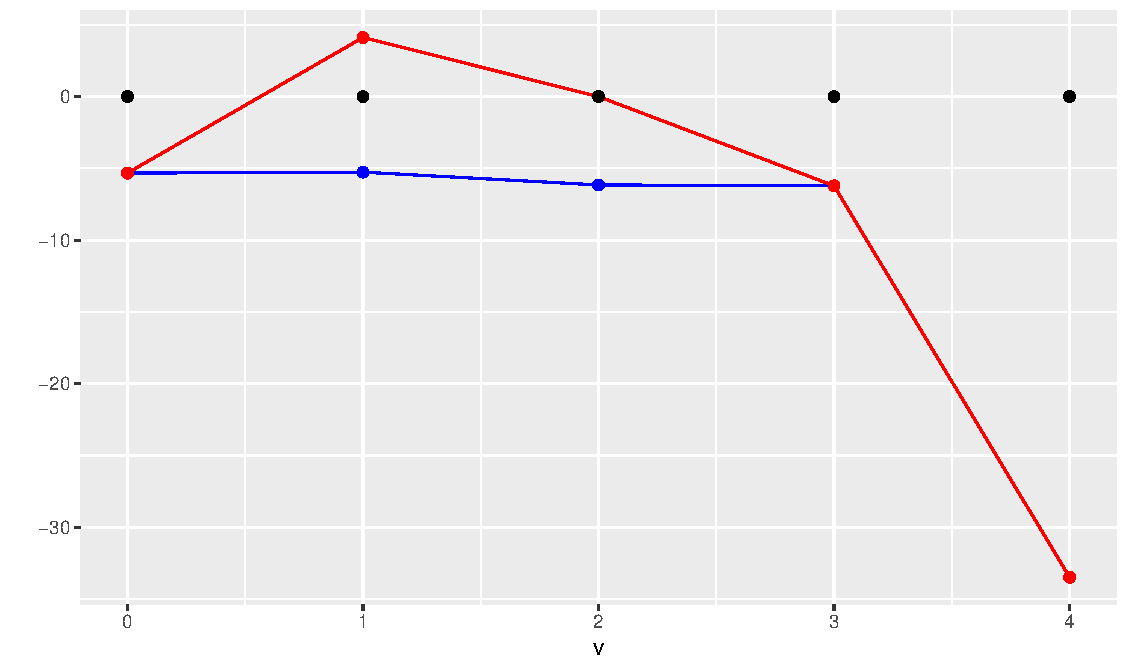
\includegraphics[scale=0.6]{plot1.pdf}
%\caption{}
%\label{fig:bounds}
\end{figure}



\newpage
\paragraph{Branch and Bound method.} The first index, $i=1$, determines the branching rule:


\begin{table}[h!]
\centering
\begin{tabular}{c|ccccccc}
 & \multicolumn{3}{c}{remove} & & \multicolumn{3}{c}{keep}\\
 & \multicolumn{3}{c}{$S\subseteq V\subseteq F\setminus\{1\}$} & & \multicolumn{3}{c}{$S\cup\{1\}\subseteq V\subseteq F$}\\
\cline{2-4} \cline{6-8}
|S|+2 & $\{2,3,4\}$ & $\mathbf{\{2,3,5\}}$ & $\{3,4,5\}$ & & $\{1,2,3\}$ & $\{1,3,4\}$ & $\{1,3,5\}$ \\
|S|+1 & $\{2,3\}$ & $\{3,4\}$ & $\mathbf{\{3,5\}}$ & & & $\{1,3\}$ &  \\
\end{tabular}
\end{table}

In the "remove" branch, the lower bound remains the same, as the sum of the last $v$ columns of $M$ is not affected by the removal of the first column. However, the upper bound changes in both branches, as the elements corresponding to $i=1$ (in $I$) are removed.






\end{document}